\documentclass{ti2}

% Dateikodierung ist utf8
\usepackage[utf8]{inputenc}   
\usepackage{graphicx}
\usepackage{listings}
\usepackage{rotating}
\usepackage{nonfloat}
\lstset{
  numbers=left,
  numberstyle=\tiny,
  breaklines=true  
}

\begin{document}

% Nr, Abgabedatum, Gruppenleiter, Gruppenname, Name1...Name4
\Abgabeblatt{3}{21.11.2016}{Marc/Bingbin}{C05}%
                {Tabea Eggers}{Jan Fiedler}%
                {Florian Pflüger}{Jonas Schmutte}%

%\begin{listing}{1}
%\begin{listingcont}

\section*{Aufgabe 1}
Beim Start gibt es einen Page-fault, weil ls nicht geladen ist, dies löst eine Trap aus, welche einen Interrupt auslöst, der einen Leseauftrag an die Platte sendet. Sobald fertig geladen ist, wird ein Interrupt ausgelöst, dass die Platte fertig ist, nun wird ein Signal gesendet, dass der Prozess abgearbeitet werden kann.%4

Dann muss die Systemuhr weitergestellt werden, dies löst einen Interrupt aus. %1

ls löst einen Page-Fault und damit eine Trap aus, da es Bereiche des Speichers einlesen will, die nicht im Hauptspeicher vorhanden sind, dies löst einen Interrupt aus, der einen Leseauftrag an die Platte sendet. Sobald fertig geladen ist, wird ein Interrupt ausgelöst, dass die Platte fertig ist, nun wird ein Signal gesendet, dass der Prozess abgearbeitet werden kann.%4

Wenn ls beginnt in die Datei Ausgabe zu schreiben, wird durch den Systemaufruf von write() gewollt eine Trap ausgelöst.

Strg-Z löst zunächst einen Interrupt aus der die eingegebenen Zeichen rettet. Nun wird das Signal SIGSTOP ausgelöst, welches ls stoppt. %2

bg löst einen Interrupt aus der die eingegebenen Zeichen rettet. Dann kommt es zu einem Page-fault welcher eine Trap auslöst, welche einen Interrupt auslöst, der einen Leseauftrag an die Platte sendet. Sobald fertig geladen ist, wird ein Interrupt ausgelöst, dass die Platte fertig ist, nun wird ein SIGCONT-Signal an den ls-Prozess gesendet, wodurch dieser fortgeführt wird. %6

Ein letzter Interrupt wird ausgelöst wenn die Platte fertig ist mit schreiben und dies meldet. %1

\section*{Aufgabe 2}

\lstinputlisting[firstline=7,firstnumber=7,lastline=34]{sigserver.cc}

\begin{minipage}{\linewidth}
	\centering%
	\tabcaption{Tests}
	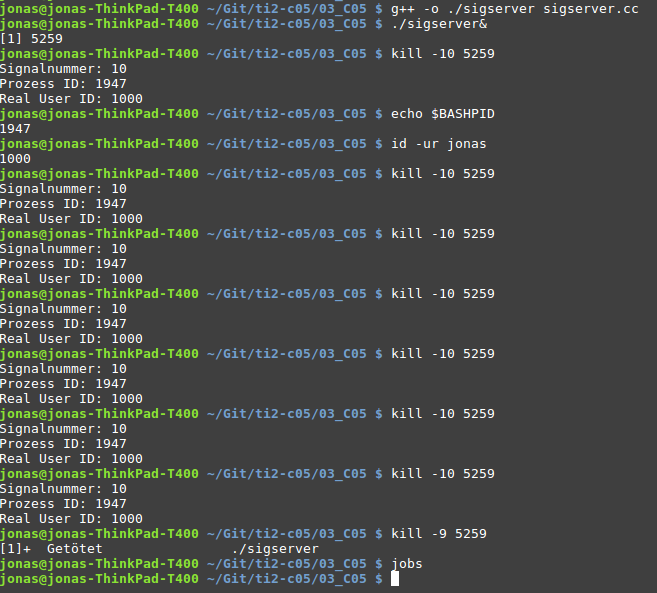
\includegraphics[width=\textwidth]{A2test.png}
\end{minipage}

Zuerst wird der Prozess gestartet und ihm ein SIGUSR1-Signal geschickt.
Seine Ausgabe gilt es zu "uberpr"ufen, Die Signalnummer ist richtig. Mit 'echo \$BASHPID' wird die ProzessID der Bash(dem hier aufrufenden Prozess) und mit 'id -ur jonas' die Real User ID des Benutzers. Diese stimmen jeweils mit der Ausgabe von 'sigserver' "uberein.

Danach wird wiederholt das SIGUSR1-Signal an den laufenden 'sigserver'-Prozess geschickt, um zu zeigen, dass er endlos auf auf Signale wartet.  

Zum Schluss schicken wir das SIGKILL-Signal an den 'sigserver'-Prozess	um zu "uberpr"ufen, dass andere Signale ihre Standardwirkung nicht verlieren. Und der Prozess wird tats"achlich get"otet.
\section*{Aufgabe 3}
zu a) \\
Wenn der CPU-Kontostand nicht halbiert werden würde, würden die Kontostände im Laufe der Zeit immer höher werden. Dies hätte zur Folge, dass auch die Prioritäten immer geringer werden würden, weil diese auch immer höher werden. Somit würden sich die Prozesse zwar immer abwechseln, aber die Prioritäten immer mehr sinken. Käme jetzt ein neuer Prozess hinzu, würde dieser immer wieder aufgerufen werden solange, bis die Priorität eines vorherigen Prozesses wieder höher ist. Kommen nun aber immer wieder neue Prozesse hinzu, werden die ersten Prozesse also nie wieder aufgerufen, da ihre Priorität zu gering ist. Im schlimmsten Fall sind diese Prozesse aber sehr wichtig und es würde somit zu Fehlern kommen, wenn diese nicht mehr aufgerufen werden. Deshalb ist es sinnvoll Prozesse 'veraltern' zu lassen.

zu b) \\
\begin{tabular}[h]{|p{2cm}||c|c|c|c|c|c|c|c|c|c|c|c|c|}
	\hline
	& 0 & 1 & 2 & 3 & 4 & 5 & 6 & 7 & 8 & 9 & 10 & 11 & 12 \\
	\hline
	\hline
	Konto A & 0 & 0 & 0 & 50 & 25 & 12 & 56 & 28 & 14 & 57 & 28 & 14 & 57 \\
	\hline
	Nutzung A & 0 & 0 & 100 & 0 & 0 & 100 & 0 & 0 & 100 & 0 & 0 & 100 & 0 \\
	\hline
	Konto A'& 0 & 0 & 50 & 25 & 12 & 56 & 28 & 14 & 57 & 28 & 14 & 57 & 28 \\
	\hline
	Prio A & 56 & 56 & 106 & 81 & 68 & 112 & 84 & 70 & 113 & 84 & 70 & 113 & 84 \\
	\hline
	\hline
	Konto B & 0 & 0 & 50 & 25 & 62 & 81 & 40 & 70 & 85 & 42 & 71 & 85 & 42 \\
	\hline
	Nutzung B & 0 & 100 & 0 & 100 & 100 & 0 & 100 & 100 & 0 & 100 & 100 & 0 & 100 \\
	\hline
	Konto B' & 0 & 50 & 25 & 62 & 81 & 40 & 70 & 85 & 42 & 71 & 85 & 42 & 71 \\
	\hline
	Prio B & 10 & 60 & 35 & 72 & 91 & 50 & 80 & 95 & 52 & 81 & 95 & 52 & 81 \\
	\hline
	\hline
	welcher Prozess läuft gerade? & - & B & A & B & B & A & B & B & A & B & B & A & B \\
	\hline
\end{tabular} \\\\
Ja, das Ergebnis lässt eine Regelmäßigkeit erkennen. Zuerst fällt auf, dass es einen Rhythmus gibt, in dem sich die Prozesse abwechseln (Prozess B läuft zwei mal, dann Prozess A, usw.). Schaut man sich dann die einzelnen Werte für einen Prozess an, fällt auf, dass diese in einem Abstand von 4 Zeitscheiben wieder in einem ähnlichen Wertebereich liegen (bei Prozess A ab 3 und bei Prozess B ab 4). \\
zu c) \\
\begin{tabular}[h]{|p{2cm}||c|c|c|c|c|c|c|c|c|c|}
	\hline
	& 0 & 1 & 2 & 3 & 4 & 5 & 6 & 7 & 8 & 9 \\
	\hline
	\hline
	Konto A & 0 & 0 & 50 & 75 & 87 & 93 & 96 & 98 & 99 & 99  \\
	\hline
	Nutzung A & 0 & 100 & 100 & 100 & 100 & 100 & 100 & 100 & 100 & 100  \\
	\hline
	Konto' A& 0 & 50 & 75 & 87 & 93 & 96 & 98 & 99 & 99 & 99  \\
	\hline
	Prio A & 0 & 50 & 75 & 87 & 93 & 96 & 98 & 99 & 99 & 99 \\
	\hline
	\hline
	Konto B & 0 & 0 & 0 & 0 & 0 & 0 & 0 & 0 & 0 & 0 \\
	\hline
	Nutzung B & 0 & 0 & 0 & 0 & 0 & 0 & 0 & 0 & 0 & 0 \\
	\hline
	Konto' B & 0 & 0 & 0 & 0 & 0 & 0 & 0 & 0 & 0 & 0 \\
	\hline
	Prio B & 99 & 99 & 99 & 99 & 99 & 99 & 99 & 99 & 99 & 99 \\
	\hline
	\hline
	welcher Prozess läuft gerade? & - & A & A & A & A & A & A & A & A & A \\
	\hline
\end{tabular} \\\\
Der Prozess B würde ab einer Basispriorität von 99 (wenn man annimmt das bei gleicher Priorität immer A die CPU bekommt, ansonsten ab einer Basispriorität von 100) nie die CPU bekommen, da Prozess A bei einer Basispriorität von 0 nicht höher als Priorität von 99 kommt. \\
zu d) \\
Annahme: Eine Zeitscheibe dauert 200ms.\\
Läuft ein Prozess wird er nicht unterbrochen. Prozess B muss also warten bis zur nächsten Zeitscheibe.\\\\
\begin{tabular}[h]{|p{2cm}||p{0.5cm}|p{0.5cm}|p{0.5cm}|p{0.5cm}|p{0.5cm}|p{0.5cm}|p{0.5cm}|p{0.5cm}|p{0.5cm}|p{0.5cm}|p{0.5cm}|p{0.5cm}|p{0.5cm}|}
	\hline
	& 0 & 1 & 2 & 3 & 4 & 5 & 6 & 7 & 8 & 9 & 10 & 11 & 12 \\
	\hline
	\hline
	Konto A & 0 & 0 & 50 & 61 & 80 & 76 & 88 & 80 & 90 & 81 & 90 & 81 & 90 \\
	\hline
	Nutzung A & 0 & 100 & 73 & 100 & 73 & 100 & 73 & 100 & 73 & 100 & 73 & 100 & 73 \\
	\hline
	Konto A'& 0 & 50 & 61 & 80 & 76 & 88 & 80 & 90 & 81 & 90 & 81 & 90 & 81 \\
	\hline
	Prio A & 0 & 50 & 61 & 80 & 76 & 88 & 80 & 90 & 81 & 90 & 81 & 90 & 81 \\
	\hline
	\hline
	Konto B & 0 & 0 & 0 & 13 & 6 & 16 & 8 & 17 & 8 & 17 & 8 & 17 & 8 \\
	\hline
	Nutzung B & 0 & 0 & 27 & 0 & 27 & 0 & 27 & 0 & 27 & 0 & 27 & 0 & 27 \\
	\hline
	Konto B' & 0 & 0 & 13 & 6 & 16 & 8 & 17 & 8 & 17 & 8 & 17 & 8 & 17 \\
	\hline
	Prio B & 15 & 15 & 28 & 21 & 31 & 23 & 32 & 23 & 32 & 23 & 32 & 23 & 32 \\
	\hline
	
\end{tabular}
\end{document}
